\documentclass[a4paper, 12pt, onecolumn, oneside]{scrartcl}

\usepackage[utf8]{inputenc}
\usepackage{amsmath}
\usepackage{amssymb}
\usepackage{graphicx}
\usepackage[hidelinks]{hyperref}
\usepackage{float}
\usepackage{enumitem}



\title{%
  Resumos de AC2 \\
  \large Teste Teorico 2}

\author{Tiago Almeida}
\date{\today} 

\begin{document}

\maketitle

\tableofcontents

\section{Introdução}
Escrever um pequeno overview da matéria que sai para o teste teórico 2
e o que esperar encontrar neste documento

\clearpage

\section{microcontroladores e Sistemas embebidos}

\section{Noção de Perifericos}
\subsection{Estrutura}
\subsection{Descodificação de endereços}
\subsection{Gerador de sinais de seleção}

\section{Portos I/O}
\subsection{Estrutura}
\subsection{Portos no PIC32}

\section{Técnicas de transferência de informação entre periféricos e memória}
\subsection{Programmed I/O (Programada)}
\subsection{Interrupt Driven I/O (Interrupção)}
\subsection{DMA (Acesso Direto)}

\section{Interrupções}
\subsection{Interrupções no PIC32}

\section{Timers}
\subsection{Funcionamento}
\subsection{Watchdog Timer}
\subsection{Timers no PIC32}

\section{Barramentos paralelos e Barramentos série}

\section{A Interface \hyperref[spi]{\textbf{\large{SPI}}}}
\hyperref[spi]{\textbf{SPI}} é uma interface de \textbf{alta velocidade e de curta distância} (dezenas de cm) usada para comunicar com
diversos dispositivos diferentes, como por exemplo:
\begin{itemize}
    \item Sensores de diversos tipos: temperatura, pressão, etc.
    \item Cartões de memória (MMC / SD)
    \item Circuitos: memórias, ADCs, DACs, Displays LCD (e.g.\ telemóveis),
    comunicação entre corpo de máquinas fotográficas e as lentes, \ldots
    \item Comunicação entre microcontroladores
\end{itemize}

A transferencia de dados em \hyperref[spi]{\textbf{SPI}} é ciclica, isto é, tudo o que é enviado é recebido de volta por quem enviou.
Assim, existem 3 tipos de transferência possiveis:
\begin{itemize}
    \item \textbf{Bidirecional}: são transferidos dados válidos em ambos os sentidos
    (master → slave e slave → master)
    \item \textbf{Master → slave (operação de escrita)}: master transfere dados
    para o slave, e ignora/descarta os dados recebidos
    \item \textbf{Slave → master (operação de leitura)}: master pretende ler dados do slave; 
    para isso transfere para o slave uma palavra com informação irrelevante (por exemplo 0); 
    o slave ignora/descarta os dados recebidos
\end{itemize}
\subsection{Funcionamento}
Pontos chave sobre a arquitetura do \hyperref[spi]{\textbf{SPI}}:\@
\begin{itemize}
    \item Apenas tem \textbf{1 master} mas pode ter \textbf{1 ou mais slaves}
    \item Relógio gerado e controlado pelo master
    \item Comunicação síncrona
    \item Comunicação \hyperref[fullduplex]{full-duplex}
    \item Apenas 1 slave pode ser selecionado por vez através do sinal \hyperref[ss]{SS}
    \item O master inicia e controla a transferência de dados, com a sinalização:
    \begin{itemize}
        \item \hyperref[sck]{\large\textbf{{SCK}}}: clock
        \item \hyperref[mosi]{\large\textbf{{MOSI}}}: Master Output Slave Input (SDO no
        master)
        \item \hyperref[miso]{\large\textbf{{MISO}}}: Master Input Slave Output (SDI no
        master)
        \item \hyperref[ss]{\large\textbf{{SS}}}: Slave select
    \end{itemize} 
    \item Quando o master envia um byte, o slave tambem envia um byte de volta ao mesmo tempo.
    Isso ocorre porque o SPI usa shift registers circulares para transferir dados.
    \begin{figure}[h]
        \centering
        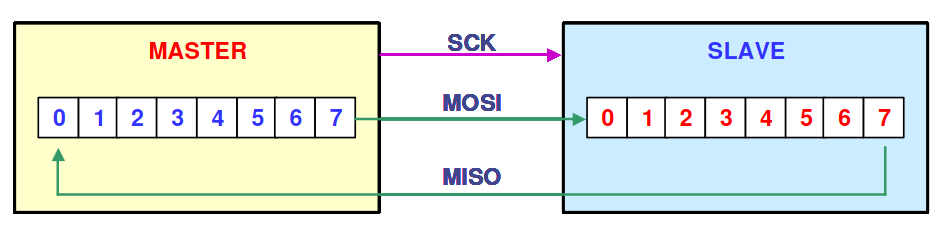
\includegraphics[width=1\textwidth]{Funcionamento_SPI.png}
        \caption{Exemplo do funcionamento do SPI}\label{fig1}
    \end{figure}
    \item Dados relevantes e Inúteis:
    \begin{itemize}
        \item Os dados que o slave envia de volta podem ou não ter significado. Se o slave não tiver dados 
        relevantes para enviar, ele pode enviar bytes preenchidos com zeros, valores padrão ou dados que não 
        são importantes para o contexto da comunicação.
    \end{itemize}
    \item Protocolo e Significado dos Dados:
    \begin{itemize}
        \item O significado dos dados trocados entre master e slave depende do protocolo de comunicação específico 
        implementado no software. O master e o slave devem ter um acordo prévio sobre o que os dados representam e 
        como devem ser interpretados.
    \end{itemize}
\end{itemize}

\clearpage
\subsection{Arquiteturas de ligação}

No caso do SPI, existem 2 arquiteturas de ligação:
\begin{itemize}
    \item \textbf{Slaves independentes}
    \item \textbf{Daisy chain}
\end{itemize}
\begin{figure}[H]
    \centering
    \begin{minipage}{0.48\textwidth}
        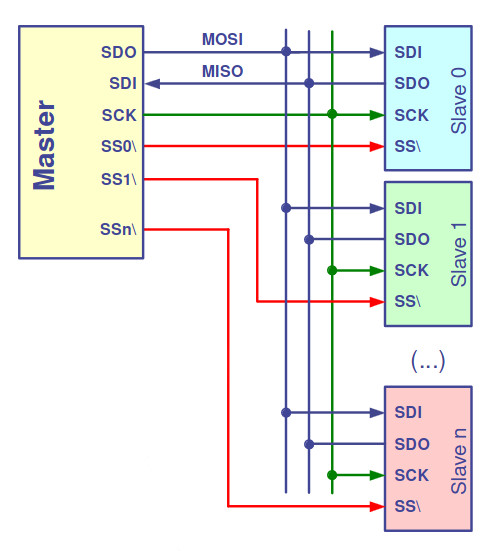
\includegraphics[width=\textwidth]{Arquitetura-de-ligação-1_SPI.jpg}
        \caption{Exemplo da arquitetura `Slaves independentes' do SPI}\label{fig2}
    \end{minipage}
    \hfill
    \begin{minipage}{0.48\textwidth}\label{fig3}
        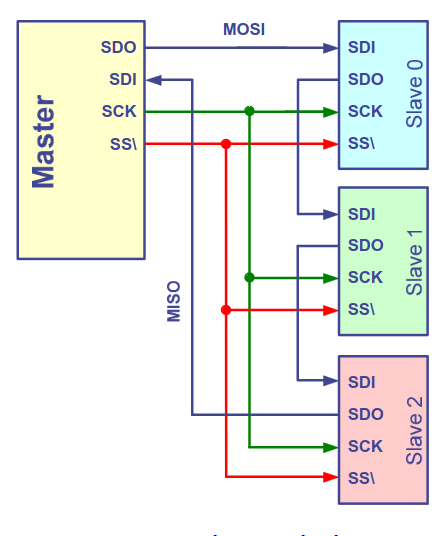
\includegraphics[width=\textwidth]{Arquitetura-de-ligação-2_SPI.png}
        \caption{Exemplo da arquitetura `Daisy chain' do SPI}
    \end{minipage}
\end{figure}

No primeiro tipo, Slaves independentes, existe no master um sinal de seleção, 
sinal \hyperref[ss]{SS} individual para cada salve.
\begin{itemize}
    \item Apenas um sinal \hyperref[ss]{SSx} pode estar ligado de cada vez
    \item O número maximo de slaves está limitado pelo numero de \hyperref[ss]{SS}
    \item O microcontrolador pode gerar, através dos seus portos digitais, sinais \hyperref[ss]{SSx} de forma a ultrapassar a limitação anterior  
\end{itemize}

\clearpage
No segundo tipo, Daisy chain, existe no master um unico sinal hyperref[ss]{SS} comum para todos os slaves.

\begin{itemize}
    \item Como podemos ver pelo fio azul do \hyperref[fig3]{exemplo de daisy chain}, a informação tem de passar
    por todos os slaves até voltar ao master, logo os slaves tem de ter a capacidade de armazenar uma sequência de N bits.
    \item Enquando o \hyperref[ss]{SS} estiver ativo, o slave ignora o comando recebido e envia para o slave seguinte ou para o master no caso do ultimo slave.
    \item O slave apenas executa o comando quando o sinal \hyperref[ss]{SS} for desativado
\end{itemize}




\subsection{Detalhes adicionais}
Algumas notas adicionais sobre \hyperref[spi]{\textbf{SPI}} que podem ou não ser importantes:

\begin{itemize}
    \item Criado pela empresa Motorola
    \item Não é exigido precisão no relógio. 
    \begin{itemize}
        \item Permite com que o se possa optar por um oscilador de baixo custo 
        \item Não é necessário um cristal de quartzo
    \end{itemize}
    \item Facil de implementar por hardware ou por software
    \item O SPI funciona sempre em modo `data exchange', isto é, o processo de comunicação 
    envolve sempre a troca do conteúdo dos shift-registers do master e do slave. 
    Cabe aos dispositivos envolvidos na comunicação usar ou descarta a informação recebida
\end{itemize}

\section{O barramento \hyperref[can]{\textbf{CAN}}}
\hyperref[can]{\textbf{CAN}} é um barramento relativamente rápido, de media distância, \textbf{adequado
para aplicação de segurança crítica devido á sua elevada robustez.} 
Alguns dos exemplos de utilização de \hyperref[can]{\textbf{CAN}} mais comuns são:
\begin{itemize}
    \item Comunicação entre subsistemas de um automóvel
    \item Aviónica, Aplicações industriais, Domótica, Robótica
    \item Equipamentos médicos, \dots
\end{itemize}

Alguns fatores que lhe dão essa robustez são:
\begin{itemize}
    \item Tolerância a interferência eletromagnética
    \item Capacidade de detetar diferentes tipos de erros
    \item Baixa probabilidade de não deteção de um erro de transmissão \\ ($4.7\times10^{-11}$)
\end{itemize}

\subsection{Funcionamento}
Pontos chave sobre a arquitetura do \hyperref[can]{\textbf{CAN}}:
\begin{itemize}
    \item É multi-master e todos os nós ligados ao barramento \hyperref[can]{\textbf{CAN}} são masters e podem produzir informação e iniciar uma transmissão.
    \item Transmissão sempre em `broadcast', ou seja, quando algum nó enviar informação todos os outros recebem
    \item Comunicação \hyperref[halfduplex]{Half-Duplex}
    \item Transmissão orientada ao bit
    \item Comunicação assíncrona e não há transmissão de relogio como em ISP.\\O transmissor e o recetor têm relógios
    locais independentes
    \item De forma a organizar a informação a ser transmitida dentro do barramento, cada mensagem enviada tem um ID associado que
    determina a sua prioridade
    \item Na transmissão de bits, a cada 5 bits iguais é adicionado 1 bit extra de polaridade oposta. \textbf{NÃO ENTENDI BEM O MOTIVO}
    \item Na transmissão, o CAN Transceiver do nó transforma o nivel lógico do bit em duas tensões e coloca nas linhas CAN\_H e CAN\_L
    \item Na receção, o CAN Transceiver do nó a receber transforma a diferença de tensões nas linhas em um nivel lógico novamente e 
    envia para o CAN Controller. 
\end{itemize}
\begin{figure}[H]
    \centering
    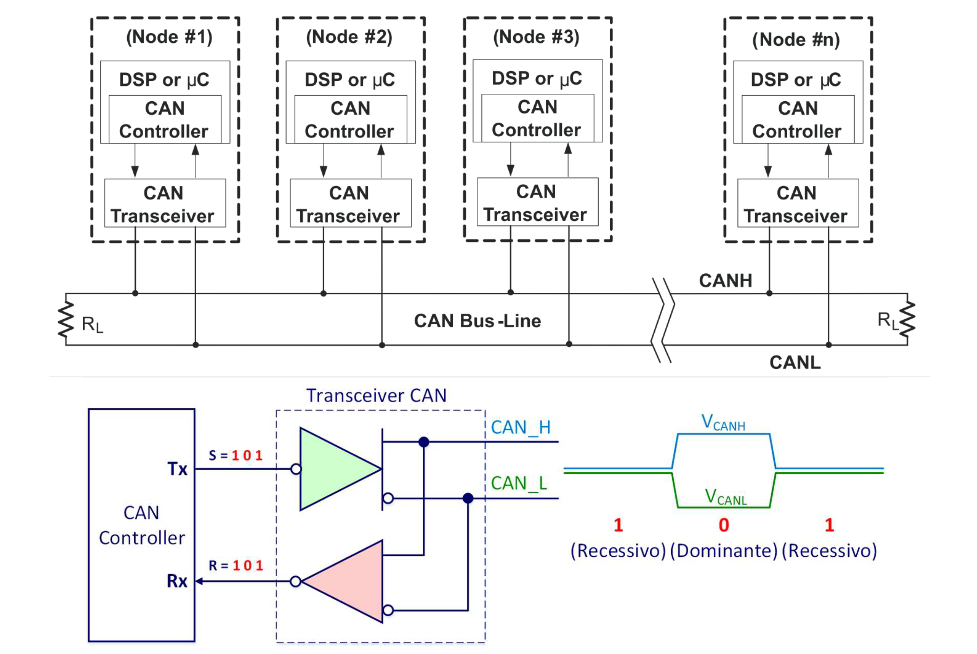
\includegraphics[width=0.9\textwidth]{Funcionamento_CAN.png}
    \caption{Exemplo do funcionamento do CAN}\label{fig4}
\end{figure}

\subsection{Formato das tramas do CAN}
O CAN envia os dados em formato de tramas, que são conjuntos de bits que carregam informação de controlo e dados.
\\Revisão de cada parte da trama:
\begin{enumerate}
    \item \textbf{SOF} (Start of Frame)
    \begin{itemize}
        \item Consiste de apenas 1 bit 
        \item Bit dominante ('0') indica o início da trama
        \item Usado para sincronizar os nós recetores
    \end{itemize}
    \item \textbf{Arbitration Field}
    \begin{itemize}
        \item Consiste de 12 bits no total
        \item Os primeiros 11 bits indicam o ID da mensagem. IDs mais baixo tem maior prioridade.
        \item O ultimo bit é o bit RTR (Remote Transmission Request). Contém o bit dominante ('0') quando a trama apenas serve para enviar dados,
        e o bit recessivo ('1') quando a trama pretende pedir informação de outros nós. O segundo caso é menos comum. 
    \end{itemize}
    \item \textbf{Control Field}
    \begin{itemize}
        \item Consiste de 6 bits no total
        \item O primeiro bit, chamado de IDE (identifier extension) serve para identificar o versão da trama CAN que se está a usar
        \item O segundo bit é reservado e não tem significado
        \item Os restantes 4 bits, chamam-se DLC (DLC3-DLC0) e indicam o numero de bytes que serão transmitidos na trama. Podem ir de 0 a 8 bytes.
    \end{itemize}
    \item \textbf{Data Field}
    \begin{itemize}
        \item Pode ter desde 0 até 8 bytes de tamanho.
        \item Contem a informação a ser transmitida
    \end{itemize}
    \item \textbf{CRC Field} (Cyclic Redundancy Check)
    \begin{itemize}
        \item Consiste de 16 bits no total
        \item Serve para deteção de erros
        \item Funciona como o checksum: Transmissor e recetor ambos calculam o valor CRC com base nos dados enviados. Se o valor calculado pelo recetor não for igual
        ao que se encontra no CRC Field (valor calculado pelo transmissor), isso indica que houve um erro.\\
    \end{itemize}
    \item \textbf{ACK Field}
    \begin{itemize}
        \item Consiste de 2 bits no total
        \item Primeiro bit é o ACK Slot: Durante a transmissão da mensagem, o transmissor envia este bit como recessivo (1). Se pelo menos um nó na rede receber a mensagem 
        corretamente, ele sobrepõe o bit recessivo com um bit dominante (0) no ACK Slot.
        \item O segundo bit é o ACK Delimiter: É um bit recessivo ('1') e serve apenas para separa o ACK do proximo campo da trama
    \end{itemize}
    \item \textbf{EOF} (End of Frame)
    \begin{itemize}
        \item Consiste em 7 bits no total
        \item Todos os bits são recessivos ('1') e indicam o fim da trama
    \end{itemize}
    \item \textbf{IFS} (Interframe/Intermission)
    \begin{itemize}
        \item Consiste em, no minimo, 3 bits no total, mas podem ser mais
        \item Todos os bits são recessivos ('1') e servem como um delay no bus para dar tempo aos nós de processar a mensagem da trama antes da proxima ser transmitida
    \end{itemize}
\end{enumerate}  

\begin{figure}[H]
    \centering
    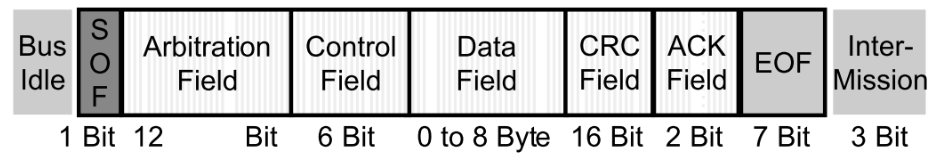
\includegraphics[width=1\textwidth]{Trama-exemplo_CAN.png}
    \caption{Exemplo da trama do CAN}\label{fig5}
\end{figure}

\subsection{Motivos da segurança adicional do CAN}
\dots

\section{A interface RS-232C}
A interface RS-232C é uma interface muito antiga e, por consequencia, simples, o que leva a que seja muito popular em microcontroladores. 

\subsection{Funcionamento}
Pontos chave sobre a arquitetura do \textbf{RS-232C}:\@
\begin{itemize}
    \item Comunicação assíncrona
    \item Comunicação Full-duplex
    \item Transmissão orientada ao byte
    \item Consiste apenas de 2 linhas de sinalização, uma de de transmissão e uma de recessão, e uma linha de Ground (voltagem = 0V)
    \item O valor enviado é codificado como a diferença entre a tensão enviada no barramento Tx e o GND.\@Se o valor for \textbf{negativo}, o valor digital enviado é 1, e se for \textbf{positivo}, o valor enviado é 0. 
    \item A descodificação é feito nos drivers de linha 
    \item A versão default desta interface apenas suporta comunicação ponto-a-ponto
\end{itemize}

\begin{figure}[H]
    \centering
    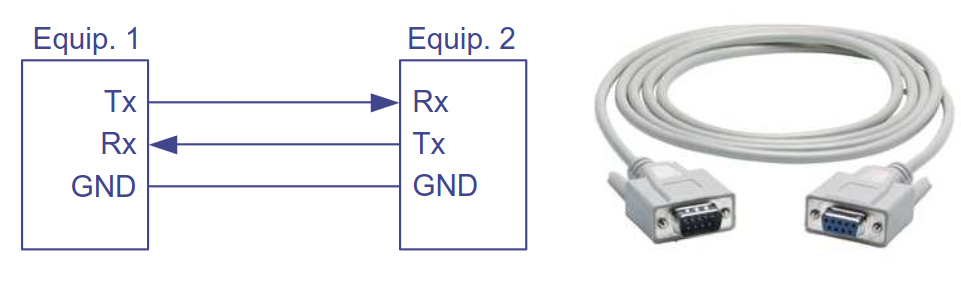
\includegraphics[width=1\textwidth]{Funcionamento_RS-232C.png}
    \caption{Exemplo do funcionamento do RS-232C}\label{fig6}
\end{figure}

\subsection{Formato das tramas do RS-232C}
O RS-232C, assim como o CAN, envia informação no formato de tramas. No entanto, tambem por ser um protocolo mais antigo
é uma trama muito mais simples em comparação.
Revisão de cada parte da trama:
\begin{enumerate}
    \item \textbf{Start bit}
    \begin{itemize}
        \item Apenas um bit com valor lógico 0 que indica o inicio da trama
        \item Tem o uso adicional de servir como ponto de sincronização para o receptor 
    \end{itemize}
    \item \textbf{Data bits}
    \begin{itemize}
        \item Consiste de 5 a 9 bits
        \item Envia os dados do menos significativo para o mais significativo\\
        Exemplo: Data = 0x0F (0000 1111); Trama: \(D_0 = 1\), \(D_1 = 1\), \(D_2 = 1\), \dots, \(D_7 = 0\)
    \end{itemize}
    \item \textbf{Parity bit} (opcional)
    \begin{itemize}
        \item Por explicar \dots
    \end{itemize}
    \item \textbf{Stop bit}
    \begin{itemize}
        \item Consiste de 1 ou 2 bits
        \item Indica o fim da trama e tem a funcionalidade adicional de servir como um `delay' entre tramas para dar tempo para processar dados
    \end{itemize}
\end{enumerate}

\begin{figure}[H]
    \centering
    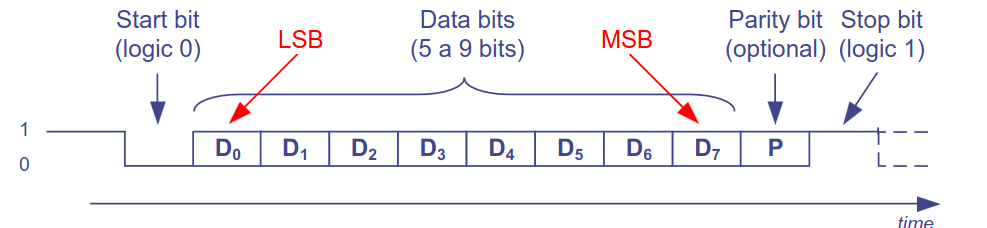
\includegraphics[width=1\textwidth]{Trama-exemplo_RS-232C.png}
    \caption{Exemplo da Trama do RS-232C}\label{fig7}
\end{figure}



\subsection{Sincronização de relógio}
Apesar da comunicação ser assincrona, porque não há transmissão de relógio, cada dispositivo envolvido (transmissor e receptor) usam o seu proprio relógio, e por isso é necessário que 
estejam sincronizados.
Para relembrar o funcionamento da sincronização reler páginas 9 a 15 da aula teorica 16.

\subsection{Máximo desvio de frequência}
\dots

\section{Device Drivers}

\section{Tecnologias de memória}
\subsection{SRAM}
\subsection{DRAM}

\section{Memória Cache}

\section{Memória Virtual}

\section{Conclusão}
Algumas conclusões e considerações que se deve ter após
ter acabado o estudo

\clearpage
\section{Glossário}\label{glossary}

Aqui está a secção de glossário. Cada termo usado repetidamente no documento está listado aqui com sua definição.

\begin{itemize}
    \item\label{spi} \textbf{SPI}: Serial Peripheral Interface
    \item\label{can} \textbf{CAN}: Controller Area Network
    \item\label{simplex} \textbf{Simplex}: comunicação apenas num sentido (TX -> RX); usada, por
    exemplo, em telemetria, para leitura remota de sensores
    \item\label{halfduplex} \textbf{Half-Duplex}: comunicação nos dois sentidos, mas apenas um de
    cada vez (é usada uma só linha)
    \item\label{fullduplex} \textbf{Full-Duplex}: Comunicação simultânea nos dois sentidos (são
    usadas duas linhas)
    \item\label{ss} \textbf{SS}: Slave select. Sinal usado pelo master para selecionar o slave. Por vezes
    tambem é usado CS (chip select) como selecionador de slave.
    \item\label{sck} \textbf{SCK}: Clock. Relógio gerado pelo master que sincroniza a transmissão/receção de dados
    \item\label{mosi} \textbf{MOSI}: Master Output Slave Input (SDO no master).
    Linha do master para envio de dados para o slave
    \item\label{miso} \textbf{MISO}: Master Input Slave Output (SDI no master).
    Linha do slave para enviar dados para o master
\end{itemize}

\end{document}
